% Harus dimuat terlebih dahulu, digunakan agar file PDF memiliki format karakter yang benar.
% Untuk informasi lebih lanjut, lihat https://ctan.org/pkg/cmap.
\RequirePackage{cmap}

% Format dokumen sebagai paper konferensi menggunakan aturan IEEEtran terbaru (v1.8b).
% Untuk informasi lebih lanjut, lihat http://www.michaelshell.org/tex/ieeetran/.
\documentclass[conference]{IEEEtran}

% Format encoding font dan input menjadi 8-bit UTF-8.
\usepackage[T1]{fontenc}
\usepackage[utf8]{inputenc}
\usepackage{amsmath}
% Digunakan untuk mengatur margin dokumen.
\usepackage{textcomp}

% Digunakan untuk tujuan demonstrasi.
\usepackage{mwe}

% Digunakan untuk menampilkan font dengan style yang lebih baik.
\usepackage[zerostyle=b,scaled=.75]{newtxtt}

% Digunakan untuk menampilkan tabel dengan style yang lebih baik.
\usepackage{booktabs}
\usepackage[table,xcdraw]{xcolor}

% Digunakan untuk menampilkan gambar pada dokumen.
\usepackage{graphicx}

% Digunakan untuk menampilkan potongan kode.
\usepackage{listings}
\lstset{
  basicstyle=\ttfamily,
  columns=fixed,
  basewidth=.5em,
  xleftmargin=0.5cm,
  captionpos=b
}

\usepackage{float}
\usepackage{tabularx}
\usepackage{wrapfig}
% Digunakan agar backticks (`) dapat dirender pada PDF.
% Untuk informasi lebih lanjut, lihat https://tex.stackexchange.com/a/341057/9075.
\usepackage{upquote}

% Digunakan untuk menyeimbangkan bagian akhir dokumen dengan dua kolom.
\usepackage{balance}

% Digunakan untuk menampilkan pustaka.
\usepackage[square,comma,numbers,sort&compress]{natbib}

% Mengubah format ukuran teks pada natbib.
\renewcommand{\bibfont}{\normalfont\footnotesize}

% Jika melebihi 3 penulis dapat dilakukan linebreakend 
\makeatletter
\newcommand{\linebreakand}{%
  \end{@IEEEauthorhalign}
  \hfill\mbox{}\par
  \mbox{}\hfill\begin{@IEEEauthorhalign}
}
\makeatother

% Menambah nama penulis ketika menggunakan perintah \citet.
% Untuk informasi lebih lanjut, lihat https://tex.stackexchange.com/a/76075/9075.
\usepackage{etoolbox}
\makeatletter
\patchcmd{\NAT@test}{\else \NAT@nm}{\else \NAT@hyper@{\NAT@nm}}{}{}
\makeatother

% Digunakan untuk melakukan linewrap pada pustaka dengan url yang panjang
% jika terdapat hyphens
\usepackage[hyphens]{url}

% Digunakan untuk menambah hyperlink pada referensi.
\usepackage{hyperref}

% Menonaktifkan warna dan bookmark pada hyperref.
\hypersetup{hidelinks,
  colorlinks=true,
  allcolors=black,
  pdfstartview=Fit,
  breaklinks=true
}

% Digunakan untuk membenarkan hyperref pada gambar.
\usepackage[all]{hypcap}

% Digunakan untuk menampilkan beberapa gambar
\usepackage[caption=false,font=footnotesize]{subfig}

\usepackage{stfloats}
% nama
\newcommand{\name}{I Putu Krisna Erlangga}
\newcommand{\authorname}{Erlangga, I Putu Krisna}
\newcommand{\nickname}{Krisna}
\newcommand{\advisor}{Dr. Eko Mulyanto Yuniarno, S.T., M.T.}
\newcommand{\coadvisor}{Dr. Diah Puspito Wulandari, S.T., M.Sc.}

% identitas
\newcommand{\nrp}{5024 20 1055}
\newcommand{\advisornip}{19740907 200212 1 001}
\newcommand{\coadvisornip}{19680601 199512 1 009}
\newcommand{\email}{5024201055@student.its.ac.id}

\newcommand{\advisoremail}{ekomulyanto@ee.its.ac.id}
\newcommand{\coadvisoremail}{diah@te.its.ac.id}

% judul
\newcommand{\tatitle}{PENERJEMAH BAHASA ISYARAT INDONESIA (BISINDO) KE MEDIA SUARA MENGGUNAKAN \emph{LONG SHORT-TERM MEMORY} (LSTM) BERBASIS INTEL \emph{NEXT UNIT COMPUTING} (NUC)}
\newcommand{\engtatitle}{\emph{TRANSLATOR OF INDONESIAN SIGN LANGUAGE (BISINDO) TO VOICE MEDIA USING LONG SHORT-TERM MEMORY (LSTM) BASED ON INTEL NEXT UNIT COMPUTING (NUC)}}

% tempat
\newcommand{\place}{Surabaya}

% jurusan
\newcommand{\studyprogram}{Teknik Komputer}
\newcommand{\engstudyprogram}{Computer Engineering}

% fakultas
\newcommand{\faculty}{Teknologi Elektro dan Informatika Cerdas}
\newcommand{\engfaculty}{Intelligence Electrical and Informatics Technology}

% singkatan fakultas
\newcommand{\facultyshort}{FTEIC}
\newcommand{\engfacultyshort}{ELECTICS}

% departemen
\newcommand{\department}{Teknik Komputer}
\newcommand{\engdepartment}{Computer Engineering}

\input{pustaka/tanda-hubung.tex}

\begin{document}

% Ubah kalimat berikut sesuai dengan judul penelitian.
\title{\engtatitle{}}

% Ubah kalimat-kalimat berikut sesuai dengan nama, institusi, alamat dan kontak penulis.
\author{
  \IEEEauthorblockN{1\textsuperscript{st} \name{}}
  \IEEEauthorblockA{\textit{dept. of \engstudyprogram{}}\\
    \textit{Institut Teknologi Sepuluh Nopember}\\
    Surabaya, Indonesia 60111\\
    \email{}}

  \and
  \IEEEauthorblockN{2\textsuperscript{nd} \advisor{}}
  \IEEEauthorblockA{\textit{dept. of \engstudyprogram{}}\\
    \textit{Institut Teknologi Sepuluh Nopember}\\
    Surabaya, Indonesia 60111\\
    \advisoremail{}}

  \linebreakand
  \IEEEauthorblockN{3\textsuperscript{rd} \coadvisor{}}
  \IEEEauthorblockA{\textit{dept. of \engstudyprogram{}}\\
    \textit{Institut Teknologi Sepuluh Nopember}\\
    Surabaya, Indonesia 60111\\
    \coadvisoremail{}}
}

% Digunakan untuk menampilkan judul dan deskripsi penulis.
\maketitle

% % Mengubah keterangan `Abstract` ke bahasa indonesia.
% % Hapus bagian ini untuk mengembalikan ke format awal.
% % \renewcommand\abstractname{Abstrak}

% \begin{abstract}

%   % Ubah paragraf berikut sesuai dengan abstrak dari penelitian.
%   \lipsum[1]


% \end{abstract}

% % Mengubah keterangan `Index terms` ke bahasa indonesia.
% % Hapus bagian ini untuk mengembalikan ke format awal.
% % \renewcommand\IEEEkeywordsname{Kata kunci}

% \begin{IEEEkeywords}

%   % Ubah kata-kata berikut sesuai dengan kata kunci dari penelitian.
%   Deep Learning

% \end{IEEEkeywords}

% Change the `Abstract` label to Indonesian.
% Remove this section to revert to the original format.
\renewcommand\abstractname{Abstract}

\begin{abstract}

  % Update the following paragraph according to the research abstract.
The deaf use sign language as their primary means of communication. According to GERKATIN, there are at least 2.9 million deaf people. This is not matched by the general public's knowledge of sign language, resulting in communication difficulties between the deaf and those around them, limiting the improvement of their quality of life. Current translator systems are still limited to word-level translation only and have not made efforts to create inclusive systems. This research developed a BISINDO translation system using the LSTM architecture. The system has been implemented on Intel NUC with the ability to translate sign movements in real-time. Users can form commonly used sentences daily and convert them into voice media with the help of control sign movements. Based on the tests conducted, the system can adapt to differences in light intensity, distance, and subjects other than the author, with the highest accuracy reaching 100\%. This system can be a solution to overcome communication barriers between the deaf and the general public.

\end{abstract}

% Change the `Index terms` label to Indonesian.
% Remove this section to revert to the original format.
\renewcommand\IEEEkeywordsname{Index terms}

\begin{IEEEkeywords}

  % Update the following keywords according to the research keywords.
  Deaf, BISINDO, LSTM, Intel NUC

\end{IEEEkeywords}


% Ubah bagian berikut sesuai dengan konten-konten yang akan dimasukkan pada dokumen
% Ubah judul dan label berikut sesuai dengan yang diinginkan.
\section{Introduction}
\label{sec:introduction}

% Ubah paragraf-paragraf pada bagian ini sesuai dengan yang diinginkan.

% Pesatnya perkembangan roket yang merupakan \lipsum[2-4]

% Pembahasan pada paper ini dimulai dengan presentasi mengenai penelitian lain (Bagian \ref{sec:penelitianterkait}).
% Kemudian dilanjutkan dengan penjelasan mengenai arsitektur dari sistem yang dibuat (Bagian \ref{sec:arsitektur}).
% Berdasarkan hal tersebut, kami menunjukkan lorem ipsum (Bagian \ref{sec:loremipsum}).
% Terakhir, didapatkan kesimpulan dari penelitian yang telah dilakukan (Bagian \ref{sec:kesimpulan}).

Sign language is a language that prioritizes manual communication by combining hand shapes, hand movement orientations, arms, lips, or facial expressions to express something. Deafness is a condition where a person cannot receive auditory stimuli through their hearing senses \cite{maulida2017}. Deaf individuals use sign language to communicate, both with other deaf individuals and the surrounding community. In Indonesia, Indonesian Sign Language (BISINDO) is more commonly used in daily life. GERKATIN notes that at least 2.9 million people, or around 1.25\% of Indonesia's total population, are deaf \cite{evitasari2015}. However, the lack of public understanding of sign language makes it difficult for deaf people to communicate, thereby limiting their quality of life.

Technological advancements today have led to various innovations that help humans in daily life, including \emph{deep learning}. One of its architectures, \emph{Long Short-Term Memory} (LSTM), can store past information and learn sequential data patterns. LSTM is ideal for translating sign language due to its sequential pattern \cite{sadli2020}. Previous research by Putri et al. successfully developed a real-time detection system for Indonesian Sign Language (BISINDO) with 65\% accuracy in 30 word classes \cite{putri2022}, while research by Suhartijo and Aljabar achieved 86\% accuracy in 10 classes using LSTM \cite{aljabar2020}.

In addition, technological advancements have also given rise to devices called \emph{mini computers}, which function like regular computers but in a smaller size with the advantages of being lightweight, compact, energy-efficient, and affordable. In 2013, Intel released a mini PC called Intel \emph{Next Unit Computing} (NUC), which provides a solution for devices with high computing capabilities and mobility \cite{minny2023}. Therefore, a system that translates Indonesian Sign Language (BISINDO) into voice media is needed as a solution to overcome communication barriers between deaf people and the general public and support GERKATIN in replacing the national sign language. The current translation system is still only implemented on laptops, so the Intel \emph{Next Unit Computing} will be the device on which the Indonesian Sign Language translation system is implemented as an initial step in creating a translation system accessible to the general public.

% Ubah judul dan label berikut sesuai dengan yang diinginkan.
% \section{Literature Review}
% \label{sec:relatedworks}

% Ubah paragraf-paragraf pada bagian ini sesuai dengan yang diinginkan.

% Update the title and label below as desired.

\section{Literature Review}
\label{sec:literaturereview}

\subsection{Previous Research}
\label{subsec:previousresearch}

Research conducted by Andi Aljabar and Suhartijo successfully translated Indonesian sign language using Convolutional Neural Network (CNN), Long Short-Term Memory (LSTM), and a combination of both architectures. Testing on 10 BISINDO vocabulary classes showed an average accuracy of 73\% for CNN, 81\% for LSTM, and 90\% for the CNN-LSTM combination \cite{aljabar2020}. Research by Husna Moetia Putri, Fadlisyah, and Wahyu Fuadi detected sign language in real-time using LSTM and MediaPipe Holistic. Evaluation on 10 BISINDO vocabularies achieved 92\% accuracy and 65\% accuracy for 30 vocabularies \cite{putri2022}. Siti Nur, Aghisna Nur Assyifa, and Habilah Nurjannah developed a BISINDO translator application using LSTM with an accuracy of 75\% on 500 data, increasing to 85\% on 1000 and 1500 data. This application has a feature to add vocabulary and save data to produce sign vocabulary output accordingly \cite{nur2023}.

\subsection{Indonesian Sign Language (BISINDO)}
\label{subsec:indonesiansignlanguage}

Deafness is the term for someone who has lost or is unable to receive auditory stimuli through their hearing senses \cite{mursita2015}. Based on birth, deafness can be divided into two: \emph{congenitally deaf} (from birth) and \emph{adventitiously deaf} (due to disease or traumatic events). Deafness is also classified based on hearing ability in decibels (dB), ranging from mild to total \cite{winarsih2007}. In Indonesia, at least 2.9 million people, or 1.25\% of the population, are deaf \cite{evitasari2015}. Deaf individuals use sign language for communication. Sign language is expressed through a combination of hand shapes, hand movement orientations, arm movements, and facial expressions \cite{mursita2015}. There are two sign languages that have developed in Indonesia: the Indonesian Sign Language System (SIBI) and Indonesian Sign Language (BISINDO). SIBI uses one hand, while BISINDO uses two. BISINDO is more commonly used because it is not bound to the structure of the Indonesian language and originates from the native language of the deaf, adapting to their understanding without emphasizing Indonesian language affixes.

\subsection{Mediapipe}
\label{subsec:mediapipe}

MediaPipe is a framework for building inference pipelines on sensory data such as audio and video. This framework enables the creation of pipelines consisting of modular components, such as inference models, media processing algorithms, and data transformations. MediaPipe abstracts and connects individual perception models into maintainable workflows, allowing components to be reused. MediaPipe's core concepts include a framework for sensory data inference, performance evaluation tools, and reusable processing components. MediaPipe is designed to support the development of machine learning and deep learning models, such as object detection and sign language movement detection \cite{lugaresi2019:}. MediaPipe Pose is a framework that can predict a total of 33 landmark locations, starting from the nose to the right leg. MediaPipe Hand is a framework that can predict 21 landmark locations covering the entire hand \cite{googleMediapipe}.

\subsection{\emph{Long Short-Term Memory} (LSTM)}
\label{subsec:lstm}

\begin{figure}[ht]
    \centering
    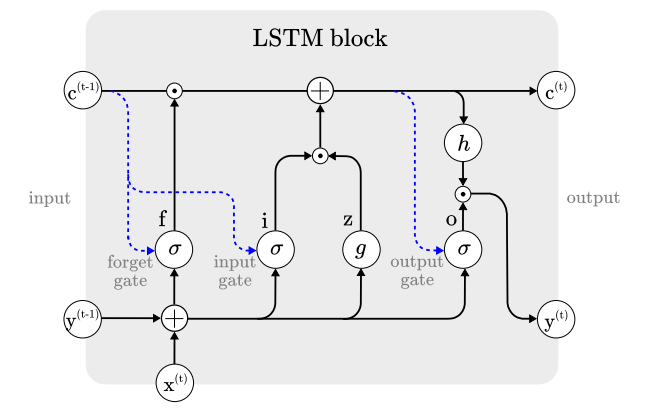
\includegraphics[scale=0.5]{gambar/bab2-lstm-model.png}
    \caption{How the LSTM architecture works}
    \label{fig:longshortterm}
\end{figure}

\emph{Long Short-Term Memory} (LSTM) is a special form of Recurrent Neural Network (RNN) that has feedback connection capabilities. This ability allows LSTM to remember information for long periods, thus solving problems with sequential or orderly characteristics. The advantage of LSTM compared to RNN is that LSTM has better and more effective memory abilities, minimizing information loss commonly occurring in processing long past information with RNN \cite{xia2020}. LSTM is very suitable for classifying sequential sign language. In Figure \ref{fig:longshortterm}, \emph{Long Short-Term Memory} is composed of several layers, including the block input, input gate, forget gate, cell, output gate, and block output, which can be sequentially formulated as follows:

\begin{equation}
    \label{eq:blockinputLSTM}
    x^{(t)} = g(W_z x^{(t)} + R_z y^{(t-1)} + b_z)
\end{equation}
\vspace{5mm}
\begin{equation}
    \label{eq:inputgateLSTM}
    i^{(t)} = \sigma(W_i x^{(t)} + R_i y^{(t-1)}+ p_i \odot c^{(t-1)} + b_i)
\end{equation}
\vspace{5mm}
\begin{equation}
    \label{eq:cellLSTM}
    c^{(t)} =  z^{(t)} \odot  i^{(t)} + z^{(t-1)} \odot  f^{(t)}
\end{equation}
\vspace{5mm}
\begin{equation}
    \label{eq:outputgateLSTM}
    o^{(t)} = \sigma(W_o x^{(t)} + R_o y^{(t-1)}+ p_o \odot c^{(t)} + b_o)
\end{equation}

\subsection{Intel \emph{Next Unit Computing} (NUC)}
\label{subsec:intelNUC}

Intel \emph{Next Unit Computing} (NUC) is a barebone computer designed by Intel. Intel NUC is a device that focuses on providing powerful computing in a practical size and can serve various user needs, from gaming to business to running complex applications. Intel NUC officially introduced this device in 2012 and marketed it publicly in early 2013 \cite{IntelNUC2020}. The first series of Intel NUC featured Sandy Bridge-based Celeron CPUs. Intel NUC has now evolved to the 12th generation, called Dragon Canyon, which features 12th generation Intel CPUs and PCI Express Gen 5 \cite{Halfacree2013}.

% Ubah judul dan label berikut sesuai dengan yang diinginkan.
% \section{Architecture}
% \label{sec:architecture}

% Update the title and label below as desired.
\section{Design and Implementation}
\label{sec:designandimplementation}

This research will 

\begin{figure}[ht]
  \centering
  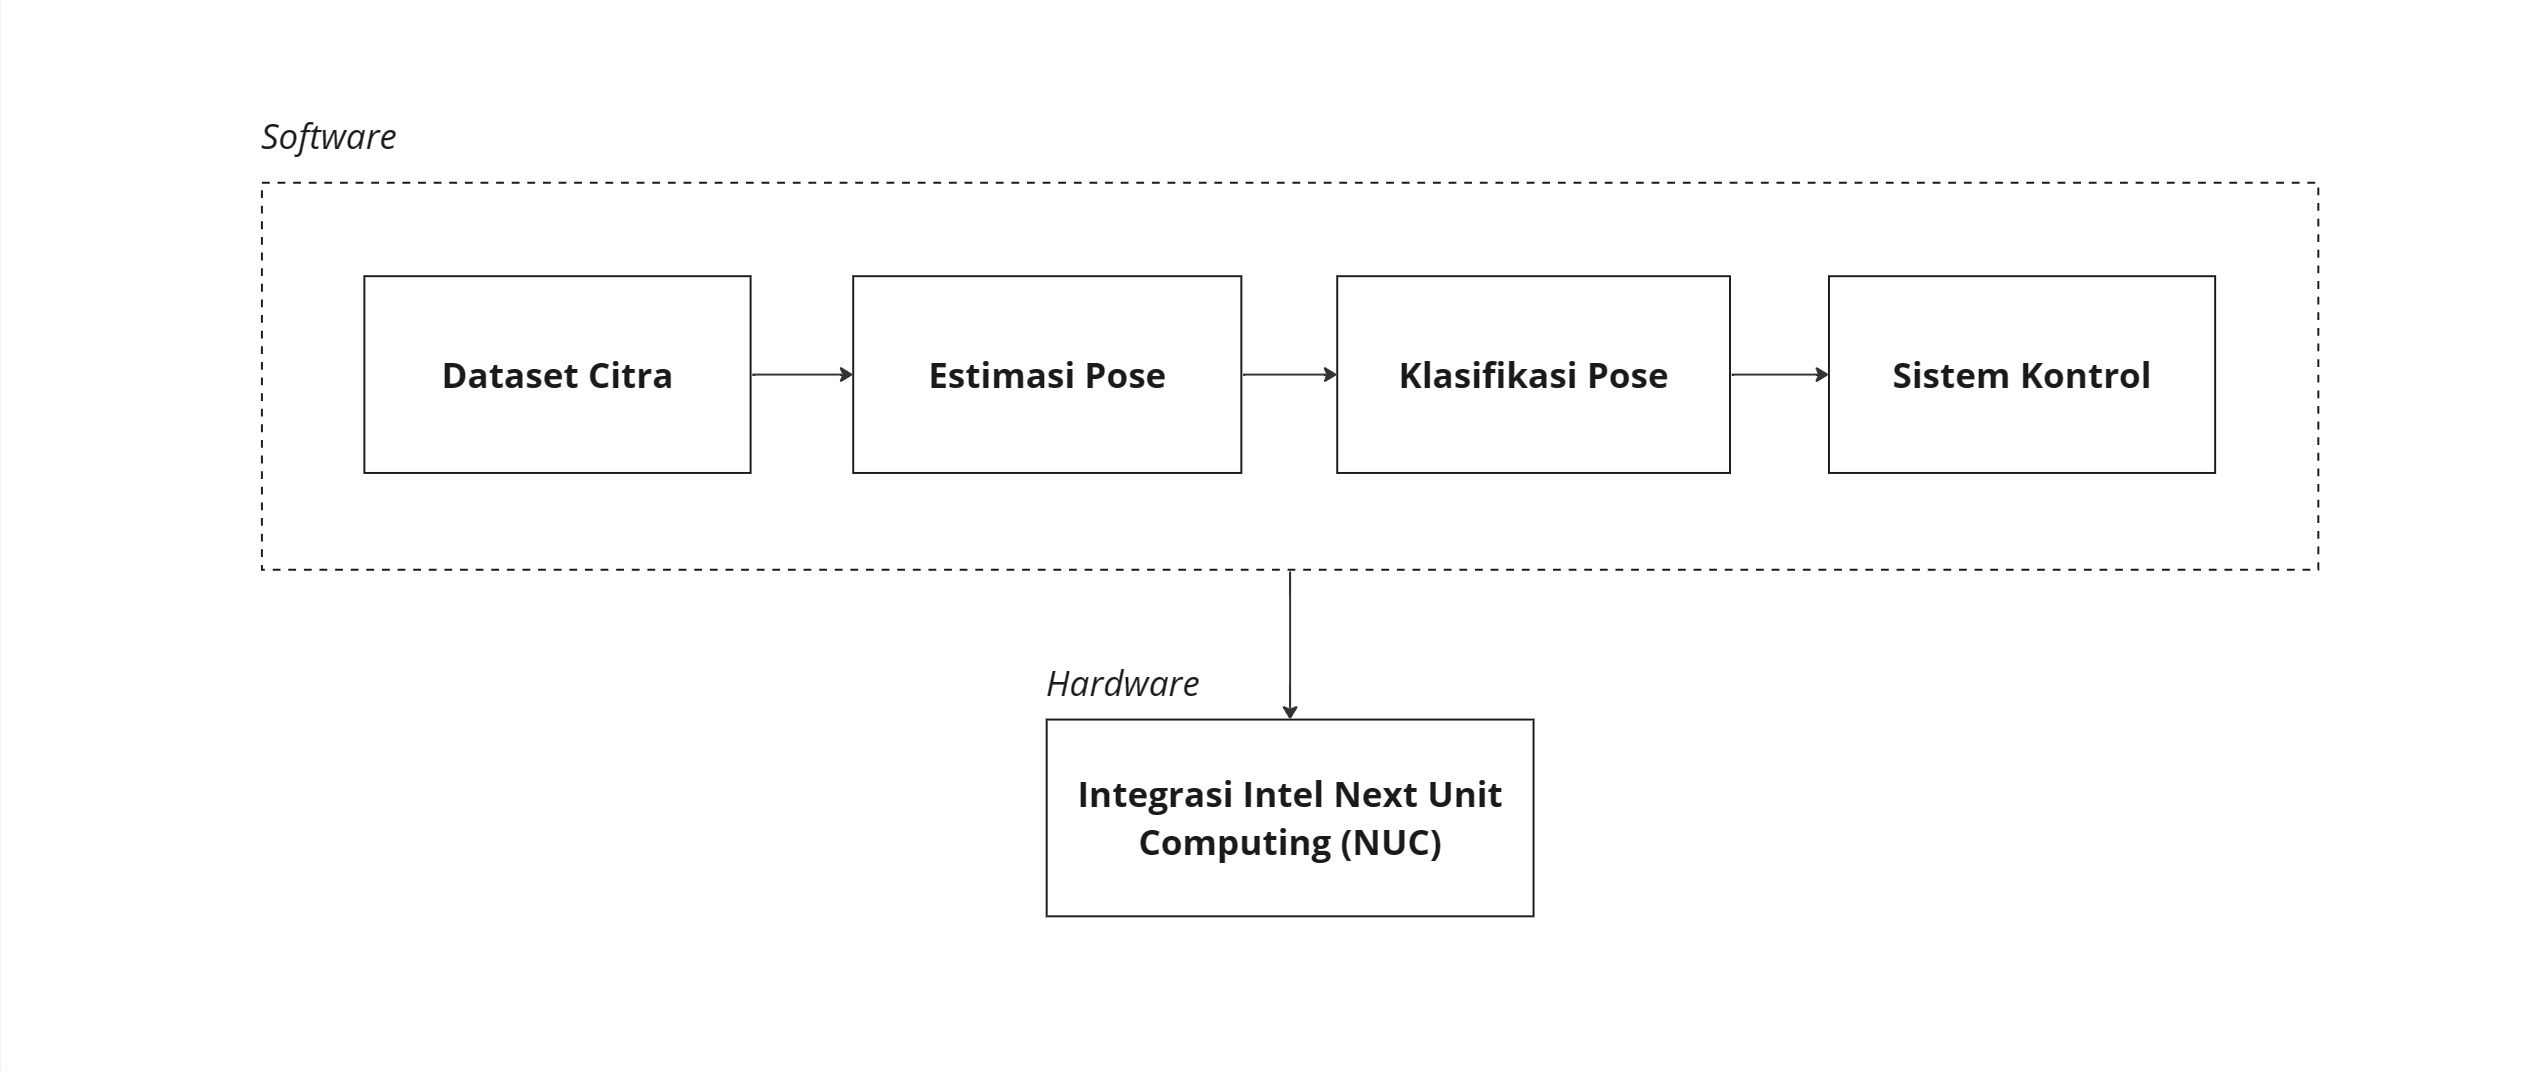
\includegraphics[scale=0.095]{gambar/bab3-block-diagram-nuc.jpg}
  \caption{Research flow}
  \label{fig:blockdiagrammethod}
\end{figure}

\subsection{Image Dataset}
\label{subsec:imagedataset}

The dataset used is a collection of images measuring 640 pixels x 480 pixels. The image data is obtained using the OpenCV library to capture video, which is then extracted into 30 frames for each data. Six BISINDO vocabulary signs with general vocabulary context and three control signs are used to facilitate system use. In sequence, the control vocabulary "standby" (indicates vocabulary transition), "delete" (deletes vocabulary), and "translate" (converts to voice).

\begin{table}[H]
  \caption{BISINDO and Control Vocabulary}
  \label{tb:kosakataBISINDO}
  \centering
  \begin{tabular}{lll}
    \toprule
    \textbf{Class} & \textbf{Data Count} & \textbf{Frame Count} \\
    \midrule
    Sorry                       & 30            & 30 \\
    Please                      & 30            & 30 \\
    I                           & 30            & 30 \\
    Name                        & 30            & 30 \\
    Home                        & 30            & 30 \\
    Who                         & 30            & 30 \\
    \textit{Standby}                       & 30             & 30 \\
    \textit{Translate}                     & 30             & 30 \\
    \textit{Delete}                        & 30             & 30 \\
    \bottomrule
  \end{tabular}
\end{table}

\subsection{Pose Estimation}
\label{subsec:poseestimation}

\begin{figure}[ht]
  \centering
  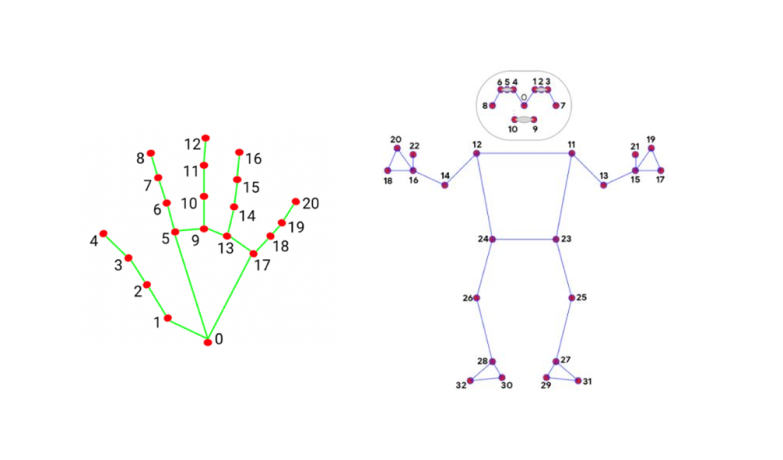
\includegraphics[scale=0.4]{gambar/bab3-pose-combine.png}
  \caption{Mediapipe Pose and Hand}
  \label{fig:estimasipose}
\end{figure}

For each image in the 30 data, pose estimation was performed with the help of the MediaPipe framework. In the formation of BISINDO signs, the moving parts of the body are the hands and arms. Through MediaPipe hand, 21 landmarks are extracted from the hand, so the total landmarks for the right and left hands are 42 landmarks. In MediaPipe pose, landmarks from the shoulder to the arm will be extracted, so the landmarks used will only be in positions 11 to 22, giving a total of 12 landmarks for the body. For each landmark, the x and y coordinates are obtained. This data is then normalized to produce a scale-invariant model (adaptable to the user's shape) and position-invariant (adaptable to the user's position). The following are the normalization formulas to be used:

\begin{equation}
  \label{eq:shouderWidthNorm}
  w = \sqrt{(x_{ka} - x_{ki})^2 + (y_{ka} - y_{ki})^2}
\end{equation}
\vspace{5mm}
\begin{equation}
  \label{eq:shoulderMidpointNorm}
  x_m = \frac{x_{ka} + x_{ki}}{2} ; \\
   y_m = \frac{y_{ka} + y_{ki}}{2}
\end{equation}
\vspace{5mm}
\begin{equation}
  \label{eq:normalization}
  x'_i = \frac{x_i - x_m}{w} ;  \\
   y'_i = \frac{y_i - y_m}{w}
\end{equation}

\subsection{Pose Classification}
\label{subsec:poseclassification}

The LSTM model used has a sequential architecture to combine a series of layers to produce a high-performing sign language translation model. The first layer is a TimeDistributed layer with a Dense layer of 128 units, 'tanh' activation, and an input shape of (30, 108), where each frame is processed independently with consistent Dense layers for each frame. The second layer is the first LSTM with 128 units, return\_sequences=True, 'tanh' activation, and an input shape of (30, 108). The third layer is a Dropout layer with a value of 0.5 to prevent excessively high weights. The fourth layer is the second LSTM with 128 units, return\_sequences=False, and 'tanh' activation, followed by a Dropout layer with a value of 0.5. To simplify the complexity of the output data from the two LSTM layers, a Dense layer with 128 units and 'relu' activation is used, followed by a Dropout layer with a value of 0.2 to prevent overfitting. The final layer is a Dense layer with 'softmax' activation and the number of units according to the number of categories. This model is compiled using the Adam optimizer and categorical crossentropy as the loss function, with categorical accuracy metrics to monitor performance during training.

\subsection{Control System}
\label{subsec:controlsystem}

The control system is a series of processes that will regulate how sign language will be detected, handle detection errors, combine various words into sentences, delete vocabulary, and translate sentences into voice. This control system is expected to facilitate the use of the translator system. The control system will be divided into two: the sign language detection program and the sentence formation program.

\newpage

\begin{figure}[H]
  \centering
  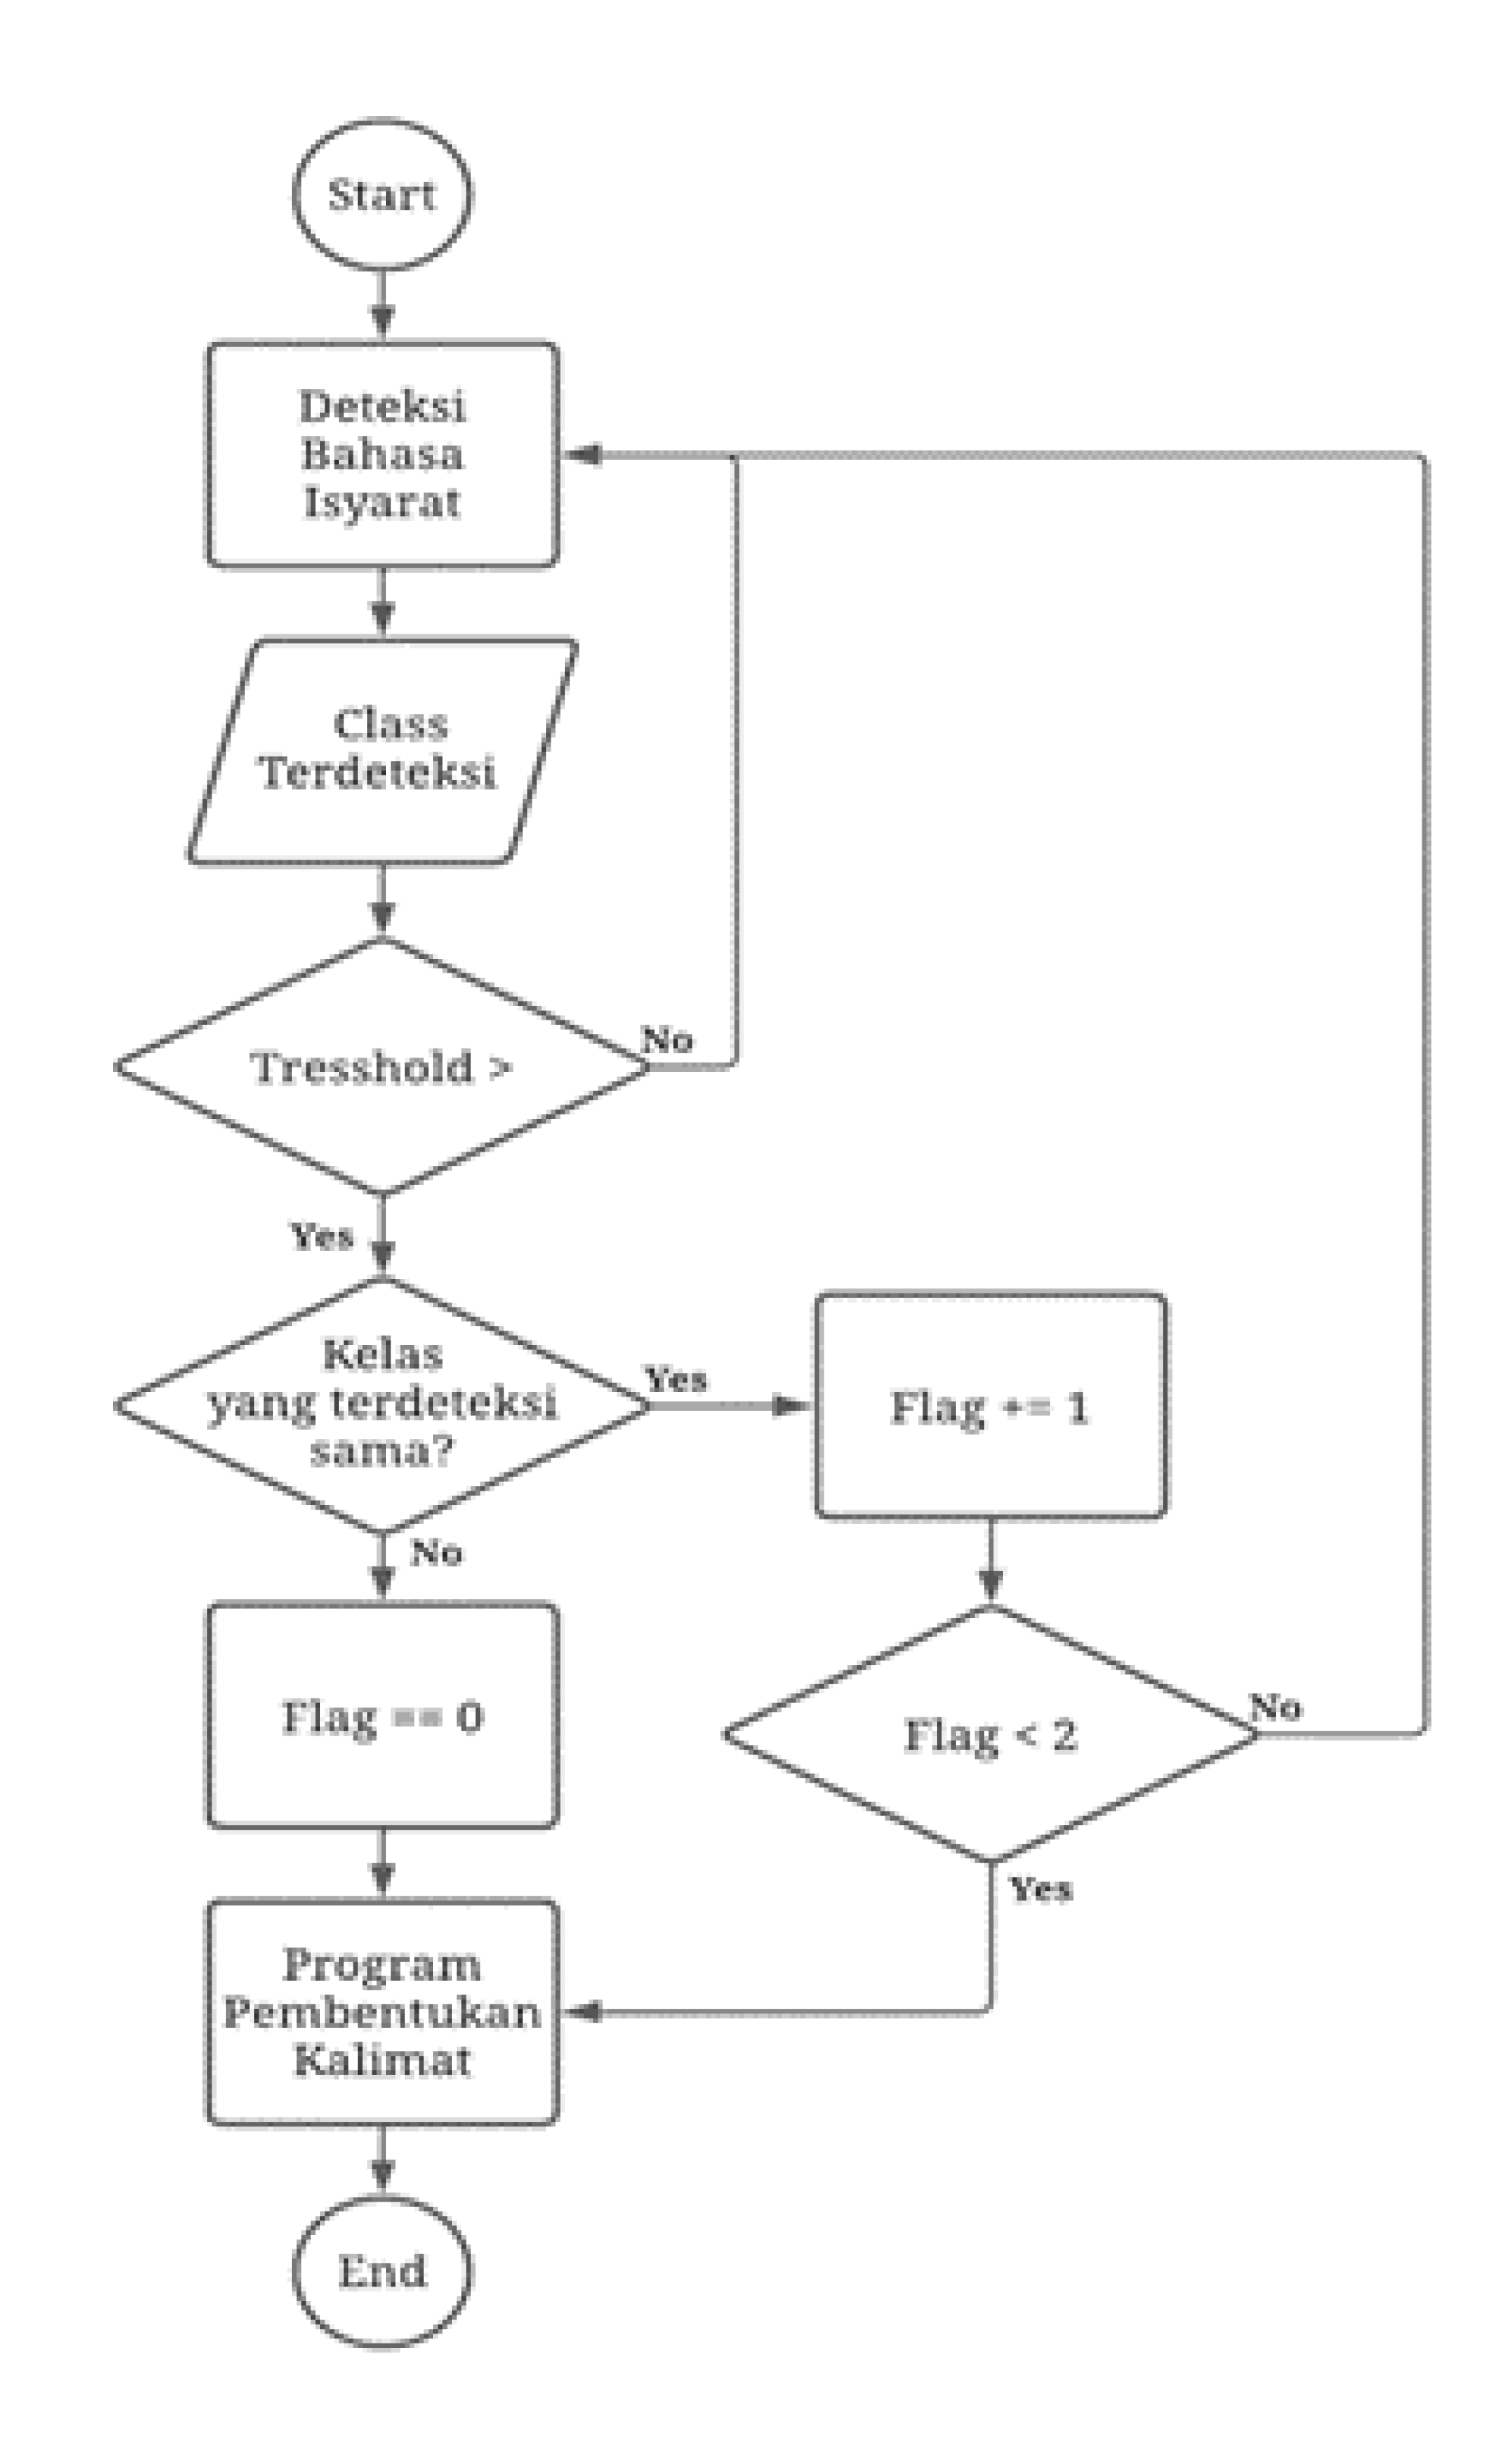
\includegraphics[scale=0.36]{gambar/bab3-flowchart-deteksi.png}
  \caption{Sign language detection program flowchart}
  \label{fig:flowchartdeteksi}
\end{figure}

\begin{figure}[H]
  \centering
  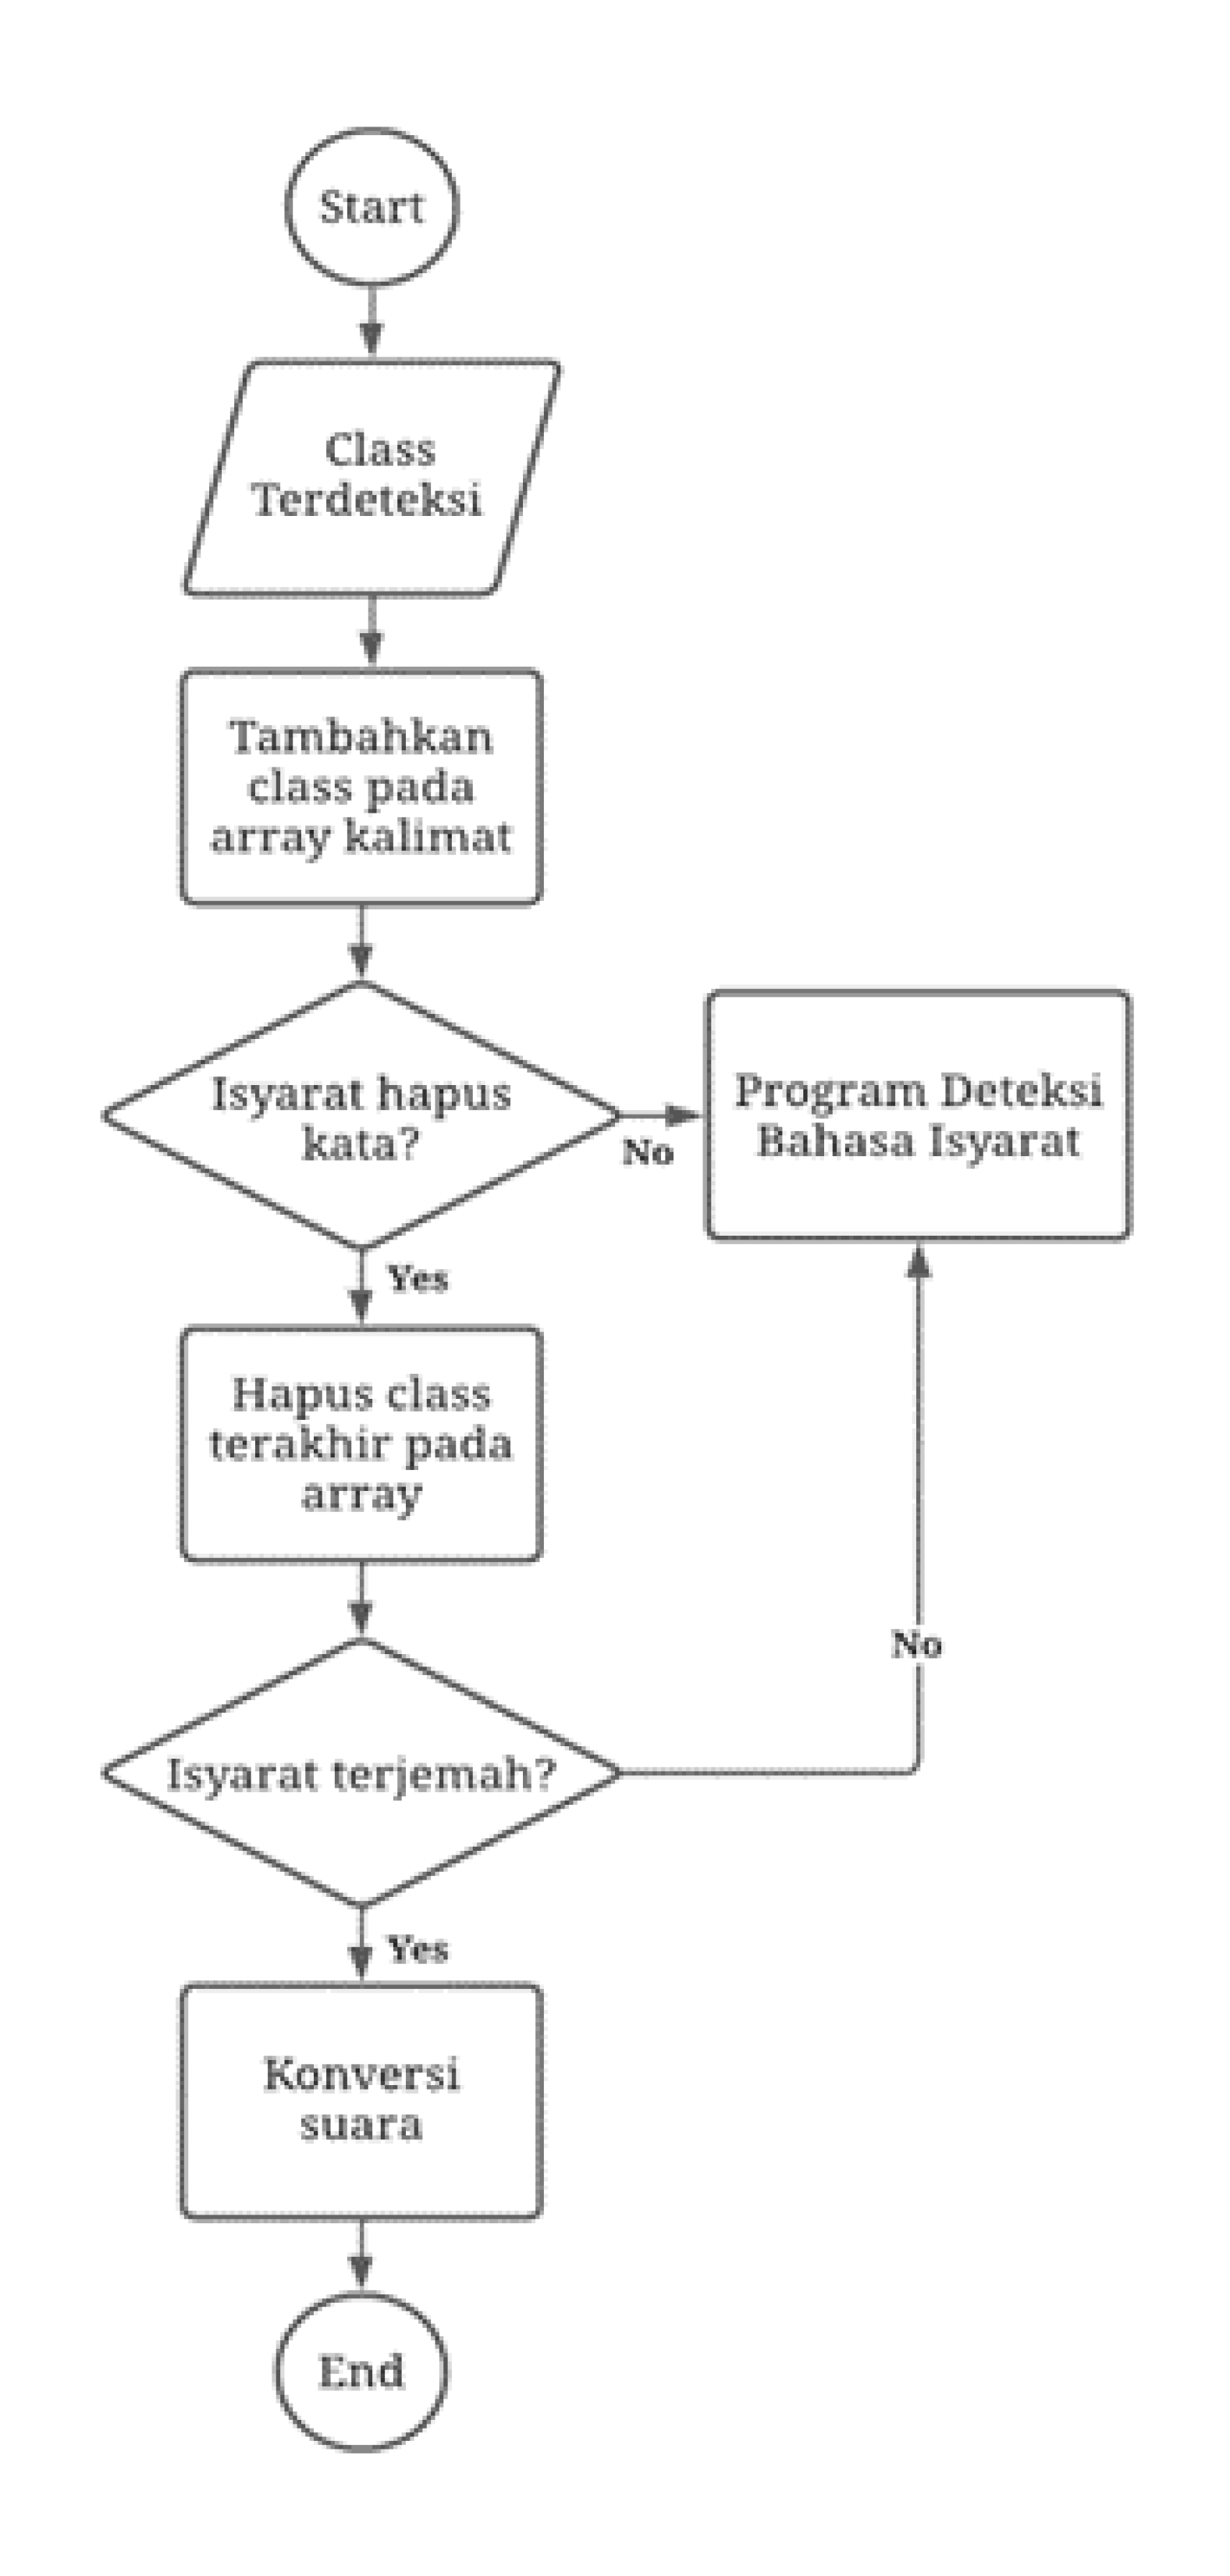
\includegraphics[scale=0.36]{gambar/bab3-flowchart-kalimat.png}
  \caption{Sentence formation program flowchart}
  \label{fig:flowchartkalimat}
\end{figure}

\subsection{Integration of \emph{Next Unit Computing} (NUC)}
\label{subsec:integrasiNUC}

Integration with Intel NUC is done by accessing a website created using the Streamlit framework, which is connected to a computer server via port forwarding. The website will access the user's webcam, allowing them to perform sign movements, which are then classified with the previously trained LSTM model in real-time.



% % Ubah paragraf-paragraf pada bagian ini sesuai dengan yang diinginkan.

% \subsection{Cetak Biru Roket}
% \label{subsec:cetakbiruroket}

% Pada cetak biru yang tertera pada Gambar \ref{fig:cetakbiru}. \lipsum[8]

% % Contoh input gambar pada kolom.
% \begin{figure} [ht]
%   \centering
%   % Ubah sesuai dengan nama file gambar dan ukuran yang akan digunakan.
%   \includegraphics[width=0.4\textwidth]{gambar/cetakbiru.jpg}

%   % Ubah sesuai dengan keterangan gambar yang diinginkan.
%   \caption{Cetak biru roket yang akan diuji coba. \cite{cetakbiruspacex}}
%   \label{fig:cetakbiru}
% \end{figure}

% \lipsum[9-10]

% \subsection{Lorem Ipsum}
% \label{subsec:loremipsum}

% \lipsum[11]

% % Contoh pembuatan tabel.
% \begin{table}
%   \caption{Contoh tabel sederhana}
%   \label{tab:tabelsederhana}
%   \centering
%   \begin{tabular}{lll}
%     \toprule
%     Heading1 & Heading2 & Heading3 \\
%     \midrule
%     One      & Two      & Three    \\
%     Four     & Five     & Six      \\
%     \bottomrule
%   \end{tabular}
% \end{table}

% % Contoh pembuatan potongan kode.
% \begin{lstlisting}[
%   language=C++,
%   caption={Program halo dunia.},
%   label={lst:halodunia}
% ]
% #include <iostream>

% int main() {
%     std::cout << "Halo Dunia!";
%     return 0;
% }
% \end{lstlisting}

% \lipsum[12]

% % Contoh pembuatan daftar.
% \begin{enumerate}
%   \item \lipsum[13][1-4]
%   \item \lipsum[13][5-8]
%   \item \lipsum[13][9-12]
% \end{enumerate}

% \lipsum[14-15]

% Ubah judul dan label berikut sesuai dengan yang diinginkan.

% % Ubah paragraf-paragraf pada bagian ini sesuai dengan yang diinginkan.

% % Contoh input beberapa gambar pada halaman.
% \begin{figure*}
%   \centering
%   \subfloat[Hasil A]{\includegraphics[width=.4\textwidth]{example-image-a}
%     \label{fig:hasila}}
%   \hfil
%   \subfloat[Hasil B]{\includegraphics[width=.4\textwidth]{example-image-b}
%     \label{fig:hasilb}}
%   \caption{Contoh input beberapa gambar.}
%   \label{fig:hasil}
% \end{figure*}

% \lipsum[16-18]

% % Contoh input potongan kode dari file.
% \lstinputlisting[
%   language=Python,
%   caption={Program perhitungan bilangan prima.},
%   label={lst:bilanganprima}
% ]{program/bilangan-prima.py}

% \lipsum[19-20]

% Update the title and label below as desired.
\section{Results and Discussion}
\label{sec:resultsanddiscussion}

% Update the paragraphs in this section as desired.

% % Example of inserting multiple images on a page.
% \begin{figure*}
%     \centering
%     \subfloat[Result A]{\includegraphics[width=.4\textwidth]{example-image-a}
%         \label{fig:resulta}}
%     \hfil
%     \subfloat[Result B]{\includegraphics[width=.4\textwidth]{example-image-b}
%         \label{fig:resultb}}
%     \caption{Example of inserting multiple images.}
%     \label{fig:result}
% \end{figure*}

% \lipsum[16-18]

% % Example of including a code snippet from a file.
% \lstinputlisting[
%     language=Python,
%     caption={Prime number calculation program.},
%     label={lst:primenumbers}
% ]{program/prime-numbers.py}

% \lipsum[19-20]

\subsection{Model Form Testing}
\label{sec:modelanalysis}
The model form tested is based on the model form explained in Subsection \ref{subsec:poseclassification}. This test was conducted to observe the impact of the LSTM model structure on the classification performance of sign language movements. The differences in the layers used are as follows:

\begin{table}[H]
    \caption{LSTM Model Structure}
    \label{tb:modelsummary}
    \centering
    \begin{tabular}{ll}
      \hline
      \textbf{Model} & \textbf{Layer Structure} \\
      \hline
      Model 1 & 
      \begin{tabular}[t]{l}
        \emph{LSTM} 1 (128 units, \emph{relu}) \\
        \emph{Dropout} 1 (0.5) \\
        \emph{LSTM} 2 (64 units, \emph{relu}) \\
        \emph{Dropout} 2 (0.5) \\
      \end{tabular} \\
      \hline
      Model 2 & 
      \begin{tabular}[t]{l}
        \emph{TimeDistributed} (\emph{Dense}, 128 units, \emph{tanh}) \\
        \emph{LSTM} 1 (64 units, \emph{tanh}) \\
        \emph{Dropout} 1 (0.5) \\
      \end{tabular} \\
      \hline
      Model 3 & 
      \begin{tabular}[t]{l}
        \emph{TimeDistributed} (\emph{Dense}, 128 units, \emph{tanh}) \\
        \emph{LSTM} 1 (128 units, \emph{tanh}) \\
        \emph{Dropout} 1 (0.5) \\
        \emph{LSTM} 2 (64 units, \emph{tanh}) \\
        \emph{Dropout} 2 (0.5) \\
      \end{tabular} \\
      \hline
    \end{tabular}
  \end{table}
  
The model is trained with 12 epochs and a dataset partition of 70:30, with 70\% training data and 30\% validation data. The trained model is then tested based on the existing test data and provides the following classification results:

\begin{table}[H]
    \caption{LSTM Model Evaluation Results}
    \label{tb:modelevaluation}
    \centering
    \begin{tabular}{lllll}
      \hline
      \textbf{Model} & \textbf{\emph{Avg. Accuracy}} & \textbf{\emph{Avg. Precision}} & \textbf{\emph{Avg. Recall}} & \textbf{\emph{Avg. F1-Score}} \\
      \hline
      Model 1 & 0.85 & 0.85 & 0.85 & 0.83 \\
      Model 2 & 0.93 & 0.95 & 0.94 & 0.94 \\
      Model 3 & 0.99 & 0.99 & 0.98 & 0.99 \\
      \hline
    \end{tabular}
  \end{table}
  
Based on Table \ref{tb:modelevaluation}, it can be seen that there is a relationship between the increased complexity of the LSTM model and the classification performance of sign language movements. This can be observed in that the third model produces the best performance with the use of a TimeDistributed layer and 2 LSTM layers.

\subsection{Light Condition Testing}
\label{sec:lightanalysis}

This test will observe the model's ability to adapt to changes in room light intensity. This test is performed using the third model tested in Table \ref{tb:modelsummary}, with the user standing 300 cm away from the camera. Light intensity data was collected using the Lux Meter application.

\begin{table}[H]
  \caption{Light Level Evaluation Results}
  \label{tb:lightevaluation}
  \centering
  \begin{tabular}{llll}
    \hline
    \textbf{Light} & \textbf{Accuracy} & \emph{\textbf{Avg. Processing Time}} & \emph{\textbf{Avg. Complete Time}} \\
    \hline
    35 lux & 0.89 & 0.0938 & 3.0335 \\
    80 lux & 0.96 & 0.0918 & 2.9928 \\
    125 lux & 1.00 & 0.0923 & 2.4777 \\
    \hline
  \end{tabular}
\end{table}

Based on Table \ref{tb:lightevaluation}, it can be seen that a reduction in light intensity in a room causes an increase in processing time and complete time. However, in terms of accuracy, the 125 lux light intensity has the best accuracy compared to other light intensities. This can be due to the camera's ability to capture the user's sign movements more clearly.

\subsection{Distance Condition Testing}
\label{sec:distanceanalysis}

This test will observe the model's ability to adapt to changes in the distance between the user and the camera. This test is performed using the third model tested in Table \ref{tb:modelsummary}, with a light intensity of 125 lux. Note that the user's sign movements should be clearly visible on the camera.

\begin{table}[H]
  \caption{Distance Evaluation Results}
  \label{tb:distanceevaluation}
  \centering
  \begin{tabular}{llll}
    \hline
    \textbf{Distance} & \textbf{Accuracy} & \emph{\textbf{Avg. Processing Time}} & \emph{\textbf{Avg. Complete Time}} \\
    \hline
    180 cm & 0.89 & 0.1017 & 2.3660 \\
    240 cm & 0.96 & 0.0994 & 2.5098 \\
    300 cm & 1.00 & 0.0997 & 2.7918 \\
    \hline
  \end{tabular}
\end{table}

Based on Table \ref{tb:distanceevaluation}, it can be seen that increasing the distance results in better model classification accuracy. This is due to the camera clearly capturing the user's sign movements as the distance increases. However, increasing the distance results in an increase in complete time, while processing time tends to be fluctuating.

\subsection{Different Subject Testing}
\label{sec:subjectanalysis}

This test is conducted to observe the model's ability to adapt to changes in subjects other than the user. This test is performed using the third model tested in Table \ref{tb:modelevaluation}, with a light intensity of 125 lux and a camera distance of 300 cm. The subjects who participated in this test can be seen in Table \ref{tb:subjectconditions}.

\begin{table}[H]
  \caption{Different Subject Variations}
  \label{tb:subjectconditions}
  \centering
  \begin{tabular}{ll}
    \hline
    \textbf{Gender} & \textbf{Subject Image} \\
    \hline
    Female & 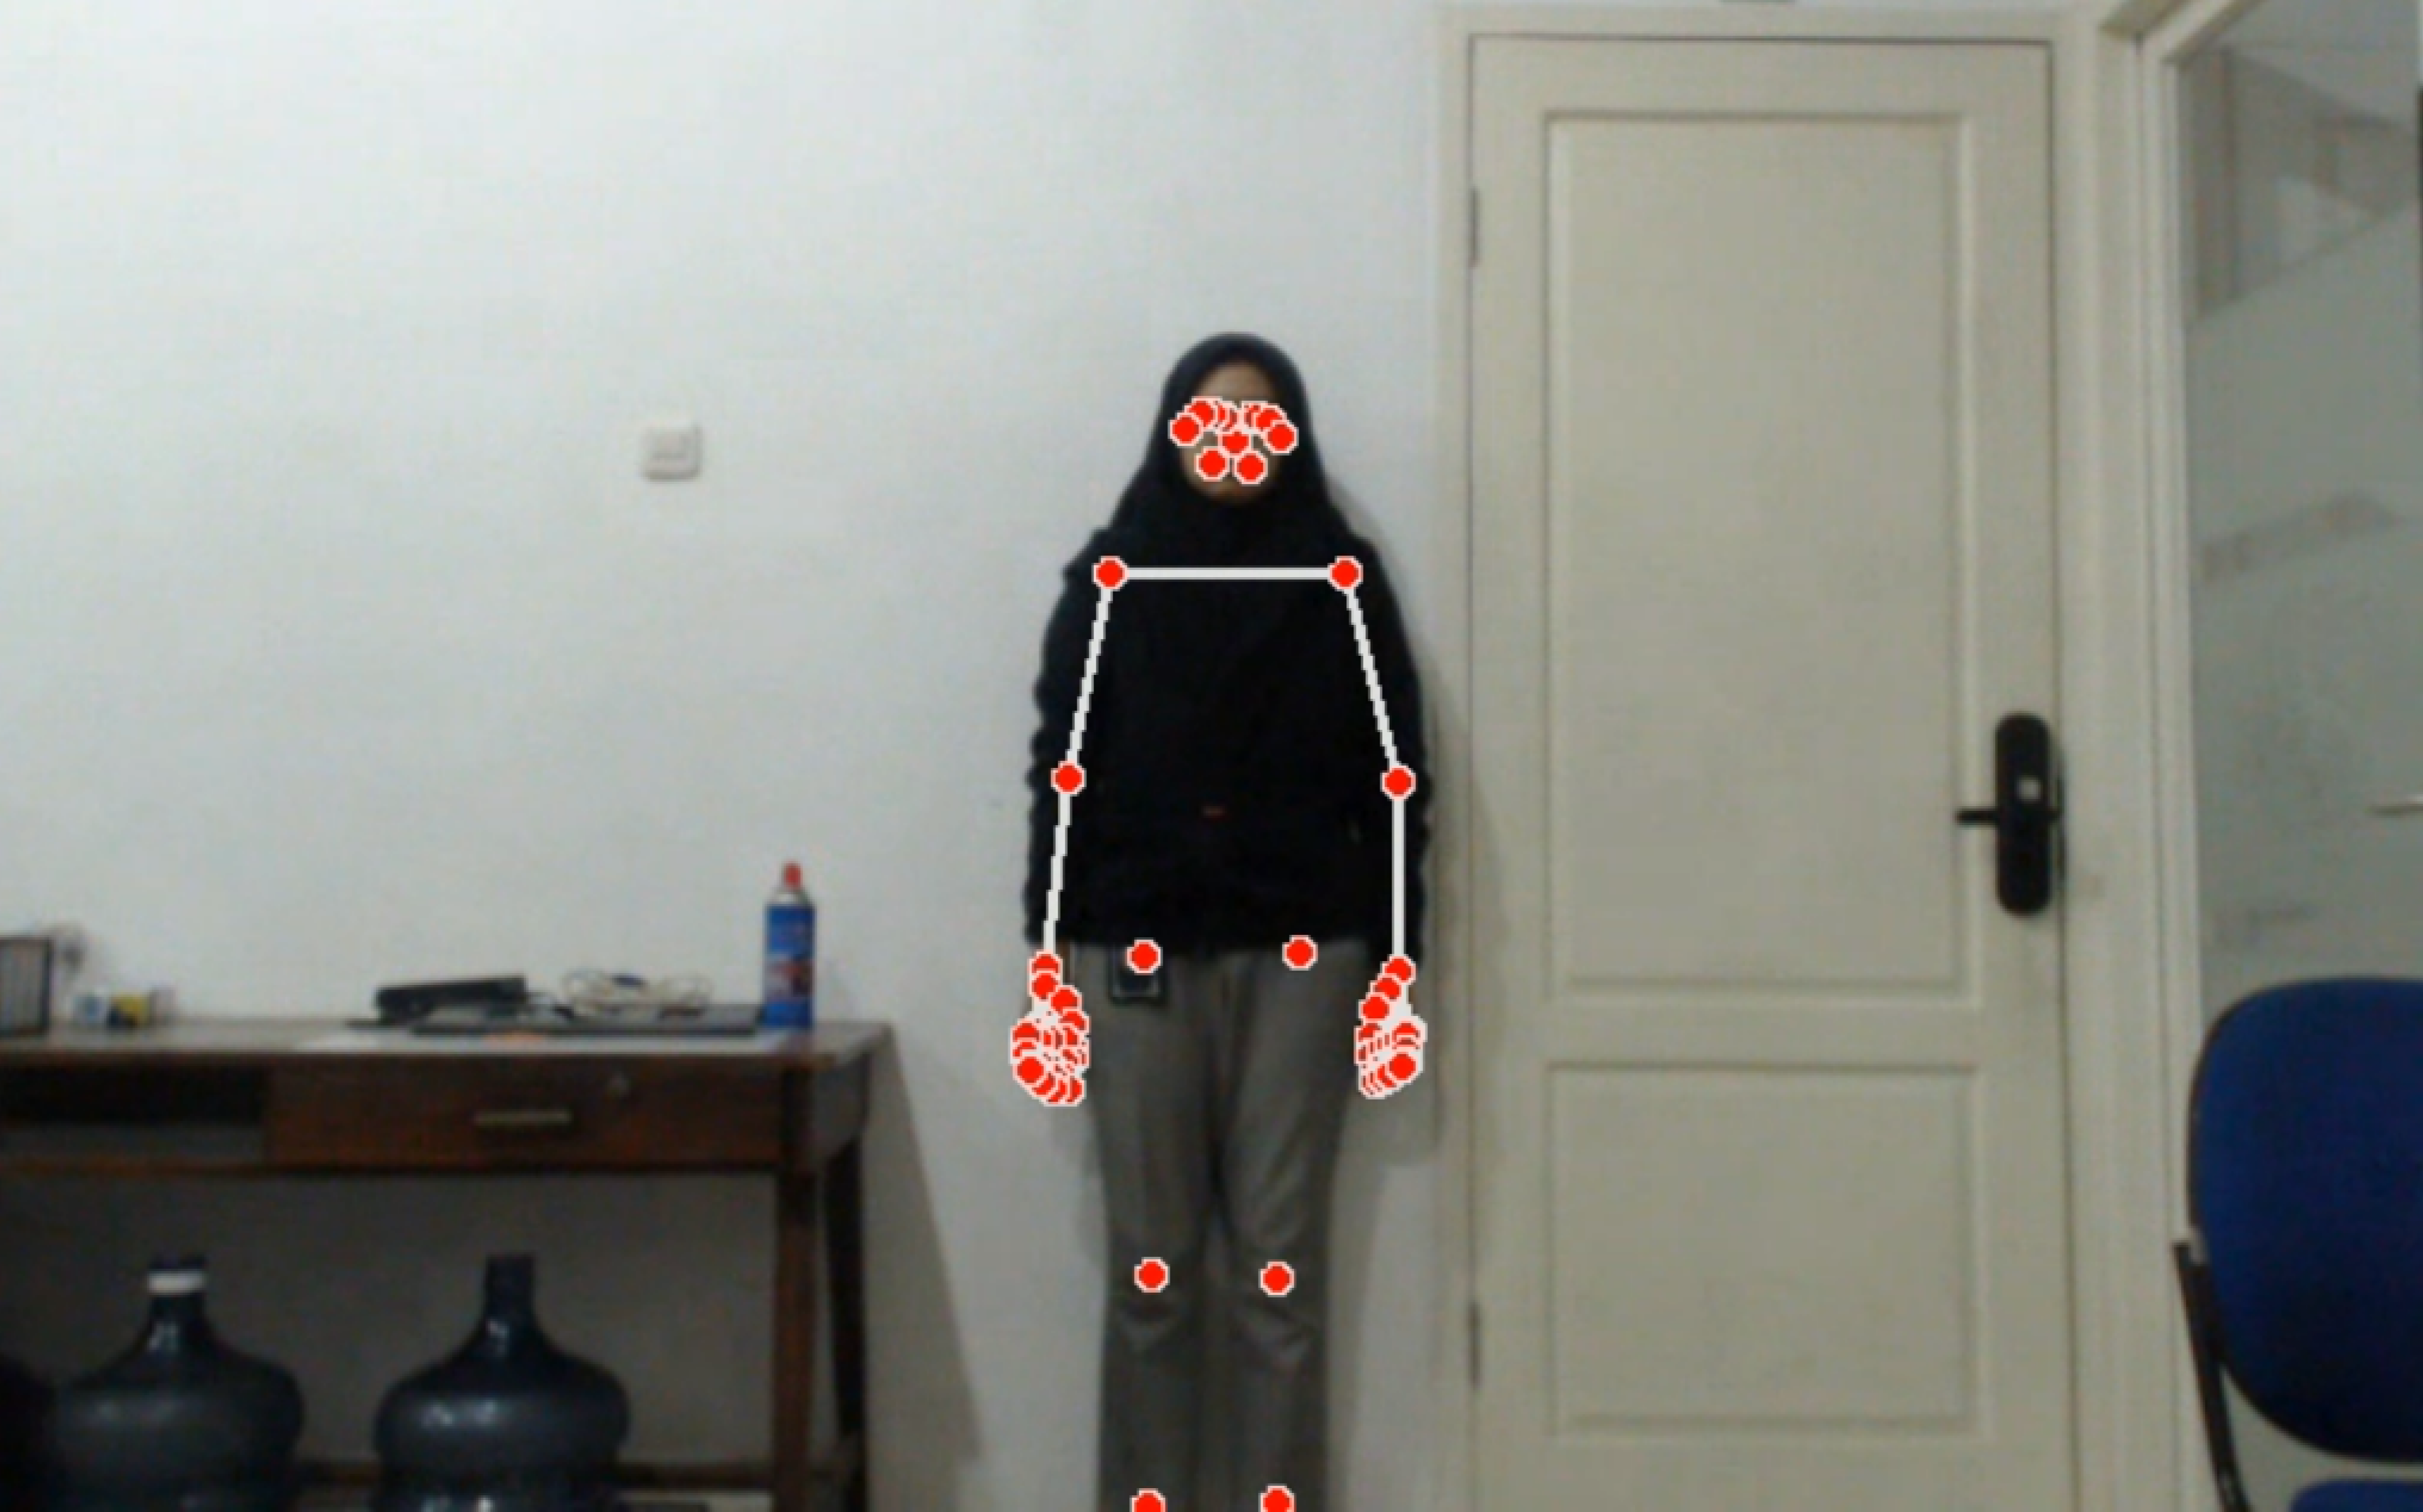
\includegraphics[scale=0.12]{gambar/bab4-rani.png} \\
    \hline
    Male & 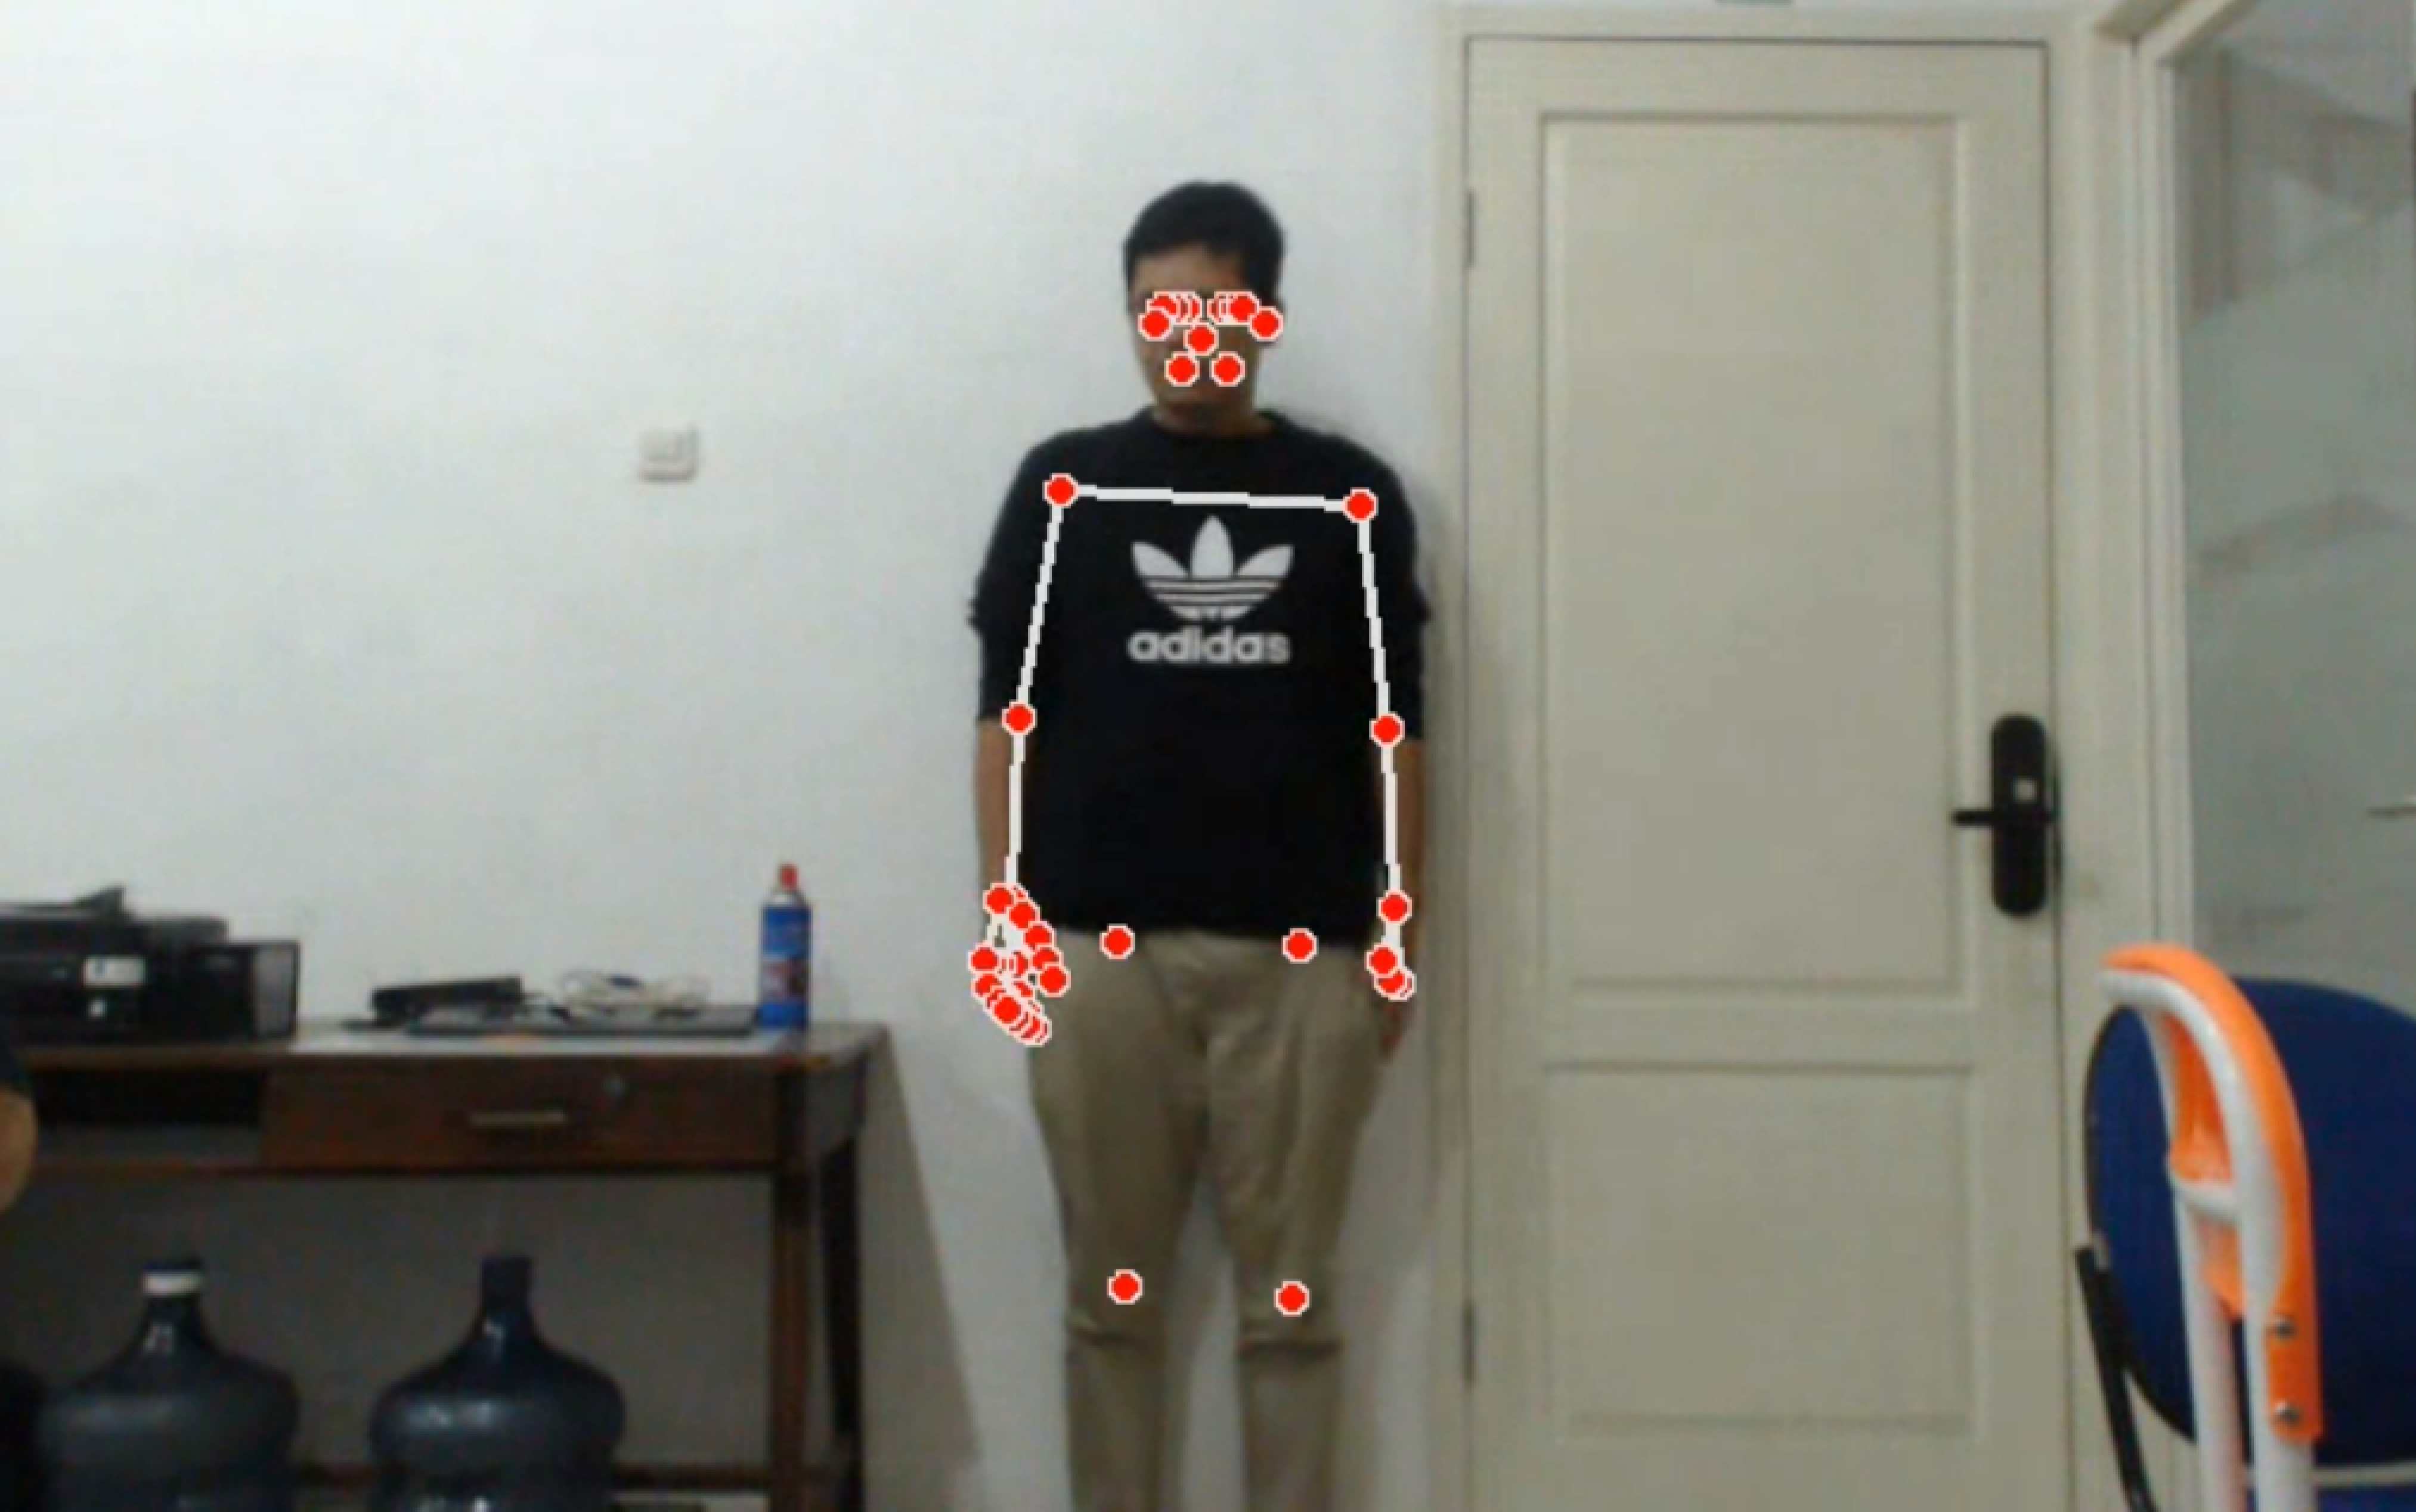
\includegraphics[scale=0.12]{gambar/bab4-evan.png} \\
    \hline
  \end{tabular}
\end{table}

\begin{table}[H]
  \caption{Different Subject Evaluation Results}
  \label{tb:subjectevaluation}
  \centering
  \begin{tabular}{llll}
    \hline
    \textbf{Subject} & \textbf{Accuracy} & \emph{\textbf{Avg. Processing Time}} & \emph{\textbf{Avg. Complete Time}} \\
    \hline
    Female & 0.93 & 0.0988 & 2.6636 \\
    Male & 0.93 & 0.0973 & 2.8191 \\
    \hline
  \end{tabular}
\end{table}

Based on Table \ref{tb:subjectevaluation}, it can be seen that the model can classify different subjects. Data normalization has resulted in a scale-invariant and position-invariant model. The model classification accuracy shows a very good value of 0.93 or 93\%. The average processing time and complete time also show values that are not much different from the previous tests, with the average processing time ranging around 0.098 and the complete time around 2.74.

\subsection{Sentence Formation and Voice Conversion Testing}
\label{sec:sentenceanalysis}

This test is conducted to understand how the translation system is used to form a series of sentences and perform voice conversion based on the formed sentences. The sentence formation in this system refers to Subsection \ref{subsec:controlsystem}. The sentences will be formed based on a combination of detected vocabulary. The full combination of vocabulary is in Table \ref{tb:vocabularycombination}. This test is performed using the third model tested in Table \ref{tb:modelevaluation}, with a light intensity of 125 lux and a camera distance of 300 cm. A maximum of three repetitions is done for each vocabulary. For each vocabulary combination, control vocabulary is also tested, including "standby," "delete," and "translate."

\begin{table}[H]
  \caption{Vocabulary and Sentence Combinations}
  \label{tb:vocabularycombination}
  \centering
  \begin{tabular}{ll}
    \hline
    \textbf{Vocabulary Combinations} & \textbf{Sentences} \\
    \hline
    "Maaf" + "Siapa" + "Nama" & "Maaf siapa nama kamu?" \\
    "Maaf" + "Tolong" + "Saya" & "Maaf tolong bantu saya" \\
    "Maaf" + "Rumah" + "Siapa" & "Maaf ini rumah siapa?" \\
    "Rumah" + "Saya" & "Ini rumah saya" \\
    "Rumah" + "Siapa" & "Ini rumah siapa?" \\
    "Siapa" + "Nama" & "Siapa nama kamu?" \\
    "Tolong" + "Saya" & "Tolong bantu saya" \\
    \hline
  \end{tabular}
\end{table}

\begin{table}[H]
  \caption{Vocabulary Combination Evaluation Results}
  \label{tb:combinationevaluation}
  \centering
  \begin{tabular}{llll}
    \hline
    \textbf{Combinations} & \textbf{Accuracy} & \emph{\textbf{Avg. Processing Time}} & \emph{\textbf{Avg. Complete Time}} \\
    \hline
    2  & 1.00 & 0.0993 & 2.8303 \\
    3  & 0.93 & 0.0981 & 2.0513 \\
    \hline
  \end{tabular}
\end{table}

As seen in Table \ref{tb:combinationevaluation}, the model has successfully formed sentences by combining them sequentially and continuously. This is shown by the accuracy of sentences formed from the combination of 2 vocabularies being 1.00 and the combination of 3 vocabularies being 0.93. The average processing time and average complete time values did not change significantly compared to the tests carried out continuously. In forming the sentence "Ini rumah saya", there was a classification error in the sign movement "home", which was classified as "delete." This is due to the high similarity between the sign movements "rumah" and "delete." Overall, the system's success rate in forming sentences is 0.857 or 85.7\%. The voice conversion process is carried out using the Google Text-to-Speech API, which has a good performance in converting sentences into voice. This also shown by the sign movement "translate" being classified as correctly within every sentence formation.

Overall, the tests show that the system has good performance in translating sign movements in relatively large numbers and in real-time.

\begin{figure}[ht]
    \centering
    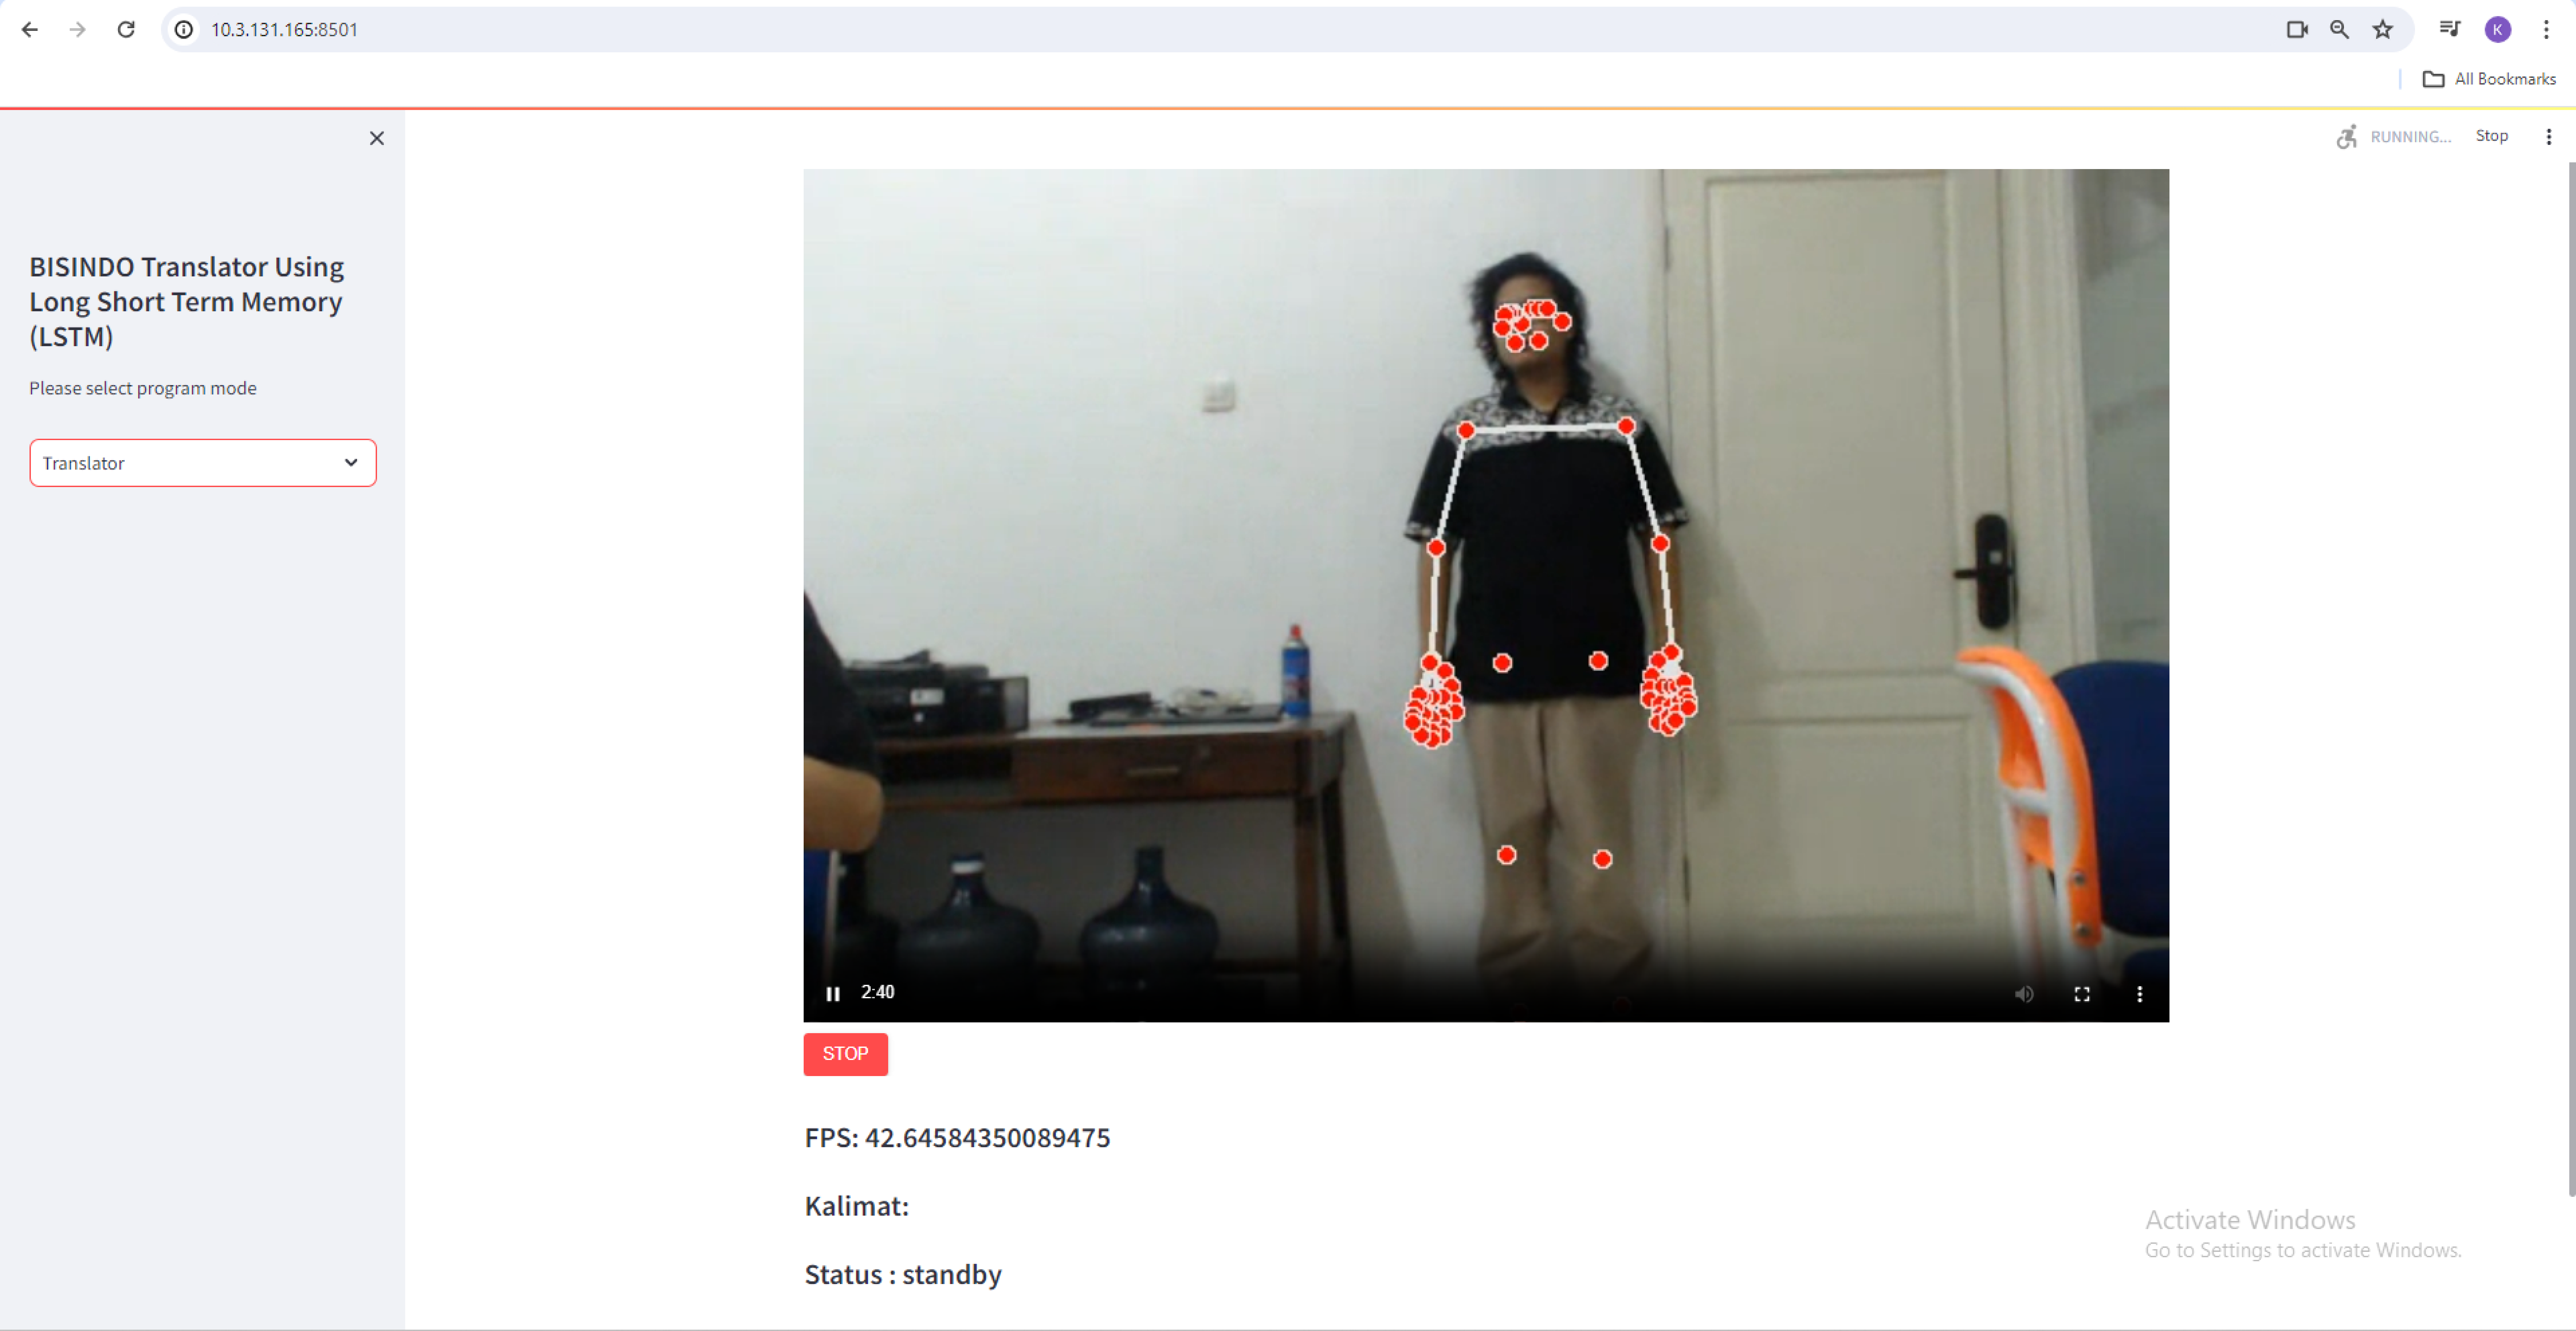
\includegraphics[scale=0.12]{gambar/bab3-layoutweb.png}
    \caption{System Testing Results}
    \label{fig:layoutweb}
\end{figure}

% Ubah judul dan label berikut sesuai dengan yang diinginkan.
\section{Conclusion}
\label{sec:conclusion}

% Ubah paragraf-paragraf pada bagian ini sesuai dengan yang diinginkan.

Based on the research conducted, the following conclusions can be drawn:

\begin{enumerate}[nolistsep]
    \item The sign language translator system has been successfully implemented on Intel \emph{Next Unit Computing} (NUC) and can operate in real-time.
    \item The LSTM model has the best performance using the \emph{TimeDistributed layer} followed by 2 LSTM layers, with an accuracy of 0.99 or 99\%.
    \item Light intensity of 125 lux or bright room conditions produces the best classification with an accuracy of 100\%.
    \item A camera distance of 300 cm from the user results in the best classification with an accuracy of 100\%.
    \item The model successfully adapts to subjects other than the author, with an accuracy of 92.5\% for both female and male subjects.
    \item The translation system can form sentences and convert them into voice with a success rate of 85.7\%.
\end{enumerate}

Based on the research conducted, the following suggestions can be considered for further development:

\begin{enumerate}[nolistsep]
  \item Adding variations in distance, light intensity, and different subjects to test how well the model can adapt to a series of changes.
  \item Consider using other methods, such as CNN-LSTM, to extract features in the form of images, allowing for better and more accurate classification of sign language movements.
\end{enumerate}


% Acknowledgment jika ada
% \input{konten/en/6-acknowledgment.tex}

% Menampilkan daftar pustaka dengan format IEEE
\bibliographystyle{IEEEtranN}
\bibliography{pustaka/pustaka.bib}

% Menyeimbangkan bagian akhir di kedua kolom
\balance

\end{document}
